\documentclass{beamer}
%\documentclass[handout]{beamer}

\mode<presentation>
{
%  \usetheme{Warsaw}
  % or ...

%  \setbeamercovered{transparent}
  % or whatever (possibly just delete it)
}


\setbeamertemplate{navigation symbols}{}

\usepackage[utf8]{inputenc}
\usepackage[spanish, es-tabla, es-nodecimaldot]{babel}
\usepackage{xcolor}


%\usepackage{times}
%\usepackage[T1]{fontenc}
% Or whatever. Note that the encoding and the font should match. If T1
% does not look nice, try deleting the line with the fontenc.


\title[Intro Prog] % (optional, use only with long paper titles)
{Introducción a la programación}

\subtitle
{Usando Python}

\author[MS]
{Mateo Suster \\ mateosuster@gmail.com}%\inst{1}}
% - Give the names in the same order as the appear in the paper.
% - Use the \inst{?} command only if the authors have different
%   affiliation.

\institute[UNGS] % (optional, but mostly needed)
{
%  \inst{1}%
  Matemática para Economistas III \\ 
  Instituto de Industria\\
  Universidad Nacional de General Sarmiento
%  \and
%  \inst{2}%
%  Department of Theoretical Philosophy\\
%  University of Elsewhere}
% - Use the \inst command only if there are several affiliations.
% - Keep it simple, no one is interested in your street address.
}

\date[] % (optional, should be abbreviation of conference name)
{ \today}



% If you have a file called "university-logo-filename.xxx", where xxx
% is a graphic format that can be processed by latex or pdflatex,
% resp., then you can add a logo as follows:

% \pgfdeclareimage[height=0.5cm]{university-logo}{university-logo-filename}
% \logo{\pgfuseimage{university-logo}}



% Delete this, if you do not want the table of contents to pop up at
% the beginning of each subsection:
%\AtBeginSubsection[]
%{
%  \begin{frame}<beamer>{Outline}
%    \tableofcontents[currentsection,currentsubsection]
%  \end{frame}
%}


% If you wish to uncover everything in a step-wise fashion, uncomment
% the following command: 

%\beamerdefaultoverlayspecification{<+->}


\begin{document}

\begin{frame}
  \titlepage
\end{frame}


\begin{frame}{Tipos de Datos y Comparaciones}
\begin{itemize}
	\item Igualdad: \texttt{i == k}\pause
	\begin{itemize}
		\item Probar \texttt{2 == 3}, \texttt{4 == 4}, \texttt{'a' == 'a'}
	\end{itemize}\pause
	\item Distinto: \texttt{i != k}\pause
	\begin{itemize}
		\item  Probar \texttt{2 != 3}
	\end{itemize}\pause
	\item Menor: \texttt{i$<$k}\pause
	\item Mayor: \texttt{i$>$k}\pause
	\item Menor o igual: \texttt{i$<=$k}\pause
	\item Mayor o igual: \texttt{i$>=$k}
\end{itemize}
\end{frame}



\begin{frame}{Tipos de Datos:  Listas}
Una \emph{lista} es una colección de valores (\textbf{definida entre corchetes}) que se acceden mediante un índice:  \pause
\\~\
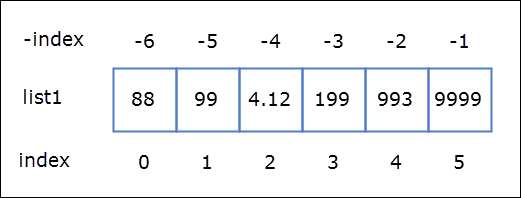
\includegraphics[width=10cm]{recursos/lista.png} \pause
\alert{Ojo, el primer elemento tiene índice 0}\pause
\\~
\alert{Y el último elemento tiene índice -1}
\end{frame}


\begin{frame}{Más sobre listas}
Algunos ejemplos de listas y operaciones:
\begin{itemize}
	\item \texttt{$[$2, 3, 5$]$} \pause 
		¿Cuál es el elemento con índice 1?\pause
	\item \texttt{$[$2, 3.5, 'cosita', 8$]$}\pause
	\item \texttt{$[$ $]$} lista vacía.\pause
	\item \texttt{c = $[$2, 3, 5$]$} define una lista de nombre \texttt{c}. \pause
	\item \texttt{$c[i]$} accede o devuelve el elemento con índice i de la lista.\pause
	\item \texttt{len(c)} devuelve la longitud de la lista.\pause
	\item \texttt{c.append(x)} agrega el elemento \texttt{x} al final de la lista \texttt{c}.
	\item Y muchas operaciones más que iremos viendo...
\end{itemize}
\end{frame}

\begin{frame}{En resumen, ¿qué es una lista?}
\pause
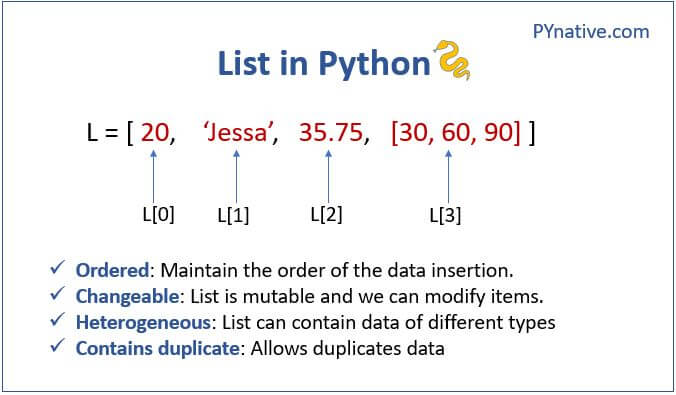
\includegraphics[width=10cm]{recursos/python_list.png} 
\end{frame}






%\section{Motivation}
%
%\subsection{The Basic Problem That We Studied}
%
%\begin{frame}{Make Titles Informative. Use Uppercase Letters.}{Subtitles are optional.}
%  % - A title should summarize the slide in an understandable fashion
%  %   for anyone how does not follow everything on the slide itself.
%
%  \begin{itemize}
%  \item
%    Use \texttt{itemize} a lot.
%  \item
%    Use very short sentences or short phrases.
%  \end{itemize}
%\end{frame}
%
%\begin{frame}{Make Titles Informative.}
%
%  You can create overlays\dots
%  \begin{itemize}
%  \item using the \texttt{pause} command:
%    \begin{itemize}
%    \item
%      First item.
%      \pause
%    \item    
%      Second item.
%    \end{itemize}
%  \item
%    using overlay specifications:
%    \begin{itemize}
%    \item<3->
%      First item.
%    \item<4->
%      Second item.
%    \end{itemize}
%  \item
%    using the general \texttt{uncover} command:
%    \begin{itemize}
%      \uncover<5->{\item
%        First item.}
%      \uncover<6->{\item
%        Second item.}
%    \end{itemize}
%  \end{itemize}
%\end{frame}
%
%
%\subsection{Previous Work}
%
%\begin{frame}{Make Titles Informative.}
%\end{frame}
%
%\begin{frame}{Make Titles Informative.}
%\end{frame}
%
%
%
%\section{Our Results/Contribution}
%
%\subsection{Main Results}
%
%\begin{frame}{Make Titles Informative.}
%\end{frame}
%
%\begin{frame}{Make Titles Informative.}
%\end{frame}
%
%\begin{frame}{Make Titles Informative.}
%\end{frame}
%
%
%\subsection{Basic Ideas for Proofs/Implementation}
%
%\begin{frame}{Make Titles Informative.}
%\end{frame}
%
%\begin{frame}{Make Titles Informative.}
%\end{frame}
%
%\begin{frame}{Make Titles Informative.}
%\end{frame}
%
%
%
%\section*{Summary}
%
%\begin{frame}{Summary}
%
%  % Keep the summary *very short*.
%  \begin{itemize}
%  \item
%    The \alert{first main message} of your talk in one or two lines.
%  \item
%    The \alert{second main message} of your talk in one or two lines.
%  \item
%    Perhaps a \alert{third message}, but not more than that.
%  \end{itemize}
%  
%  % The following outlook is optional.
%  \vskip0pt plus.5fill
%  \begin{itemize}
%  \item
%    Outlook
%    \begin{itemize}
%    \item
%      Something you haven't solved.
%    \item
%      Something else you haven't solved.
%    \end{itemize}
%  \end{itemize}
%\end{frame}
%
%
%
%% All of the following is optional and typically not needed. 
%\appendix
%\section<presentation>*{\appendixname}
%\subsection<presentation>*{For Further Reading}
%
%\begin{frame}[allowframebreaks]
%  \frametitle<presentation>{For Further Reading}
%    
%  \begin{thebibliography}{10}
%    
%  \beamertemplatebookbibitems
%  % Start with overview books.
%
%  \bibitem{Author1990}
%    A.~Author.
%    \newblock {\em Handbook of Everything}.
%    \newblock Some Press, 1990.
% 
%    
%  \beamertemplatearticlebibitems
%  % Followed by interesting articles. Keep the list short. 
%
%  \bibitem{Someone2000}
%    S.~Someone.
%    \newblock On this and that.
%    \newblock {\em Journal of This and That}, 2(1):50--100,
%    2000.
%  \end{thebibliography}
%\end{frame}

\end{document}



